\newpage
\subsection{Interview mit Dr. Hüttenhofer}

\subsubsection{Vorwort zum Interview}
Das Interview stellt den Praktischen Teil dieser Seminararbeit dar, wieso gerade ein Interview und das auch noch mit einem Politiker ist einfach zu beantworten. Ein Interview soll ja die Meinung des zu interviewten darstellen und da eine Meinung aus einer anderen Perspektive immer interessant zu hören ist und, bot sich das sehr gut an. Theoretisch hätte man auch mit jeder beliebigen Person zu diesem Thema ein Interview führen können, jedoch habe ich mich für extra dazu entschlossen unbedingt ein Interview mit einem Politiker zu führen, da dessen Meinung objektiv betrachtet um einiges interessanter ist, ein Politiker sollte ja aktiv etwas (ins positive) verändern wollen.
\begin{wrapfigure}{5}{5cm}
    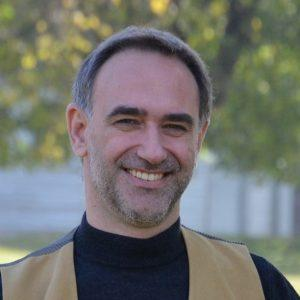
\includegraphics[width=4.5cm]{Mario.jpg}
    \caption{Mario Huettenhofer \cite{Gruene}}
\end{wrapfigure}\\
\\
Da Dr. Gritzo und Dr. Hüttenhofer sich noch aus dem Studium kannten, bot mir Dr. Gritzo an die erste Kontaktaufnahme zu übernehmen um bescheid zu geben worum es geht. Bis zum Interview blieben Dr. Hüttenhofer und ich per E-Mail in Kontakt. Das Interview fand am 15.01.2020 Im Gasthof \glqq Sonne\grqq{} um 17:00 Uhr statt und hat ca. 1 Stunde gedauert.\\
\\
Da ich zuvor noch nie einen Politiker interviewt habe, unterscheiden sich meine Erwartungen etwas, von meinem persönlichen Eindruck im positiven Sinne. Meine Erwartungen waren, dass ich ein eher unpersönliches, Fachliches Gespräch führen würde. Unpersönlich war es jedoch nicht, er hat sogar vorgeschlagen sich zu lieber "duzen", da dies das Gespräch lockerer hält. Aus formalen gründen habe ich die Fragen, jedoch in der \glqq Sie\grqq{}-Form, aufgezeichnet. Das Interview verlief sehr gut, meine Fragen wurden beantwortet und ich bekam einen guten Eindruck von Dr. Hüttenhofers allgemeinen politischen Stellung und zwar das man jetzt etwas verändern soll und es nicht verschieben soll, er hat sich hierbei aber auch vorsichtig ausgedrückt, da er weiß das es schon schwer genug ist die kleinste Kleinigkeit zu verändern. Trotzdem empfinde ich seine Stellung, als sehr vorbildlich und zukunftsorientiert, da logischerweise alles was gegenwärtig verändert wird, die Zukunft ins positive bzw. ins negative verändert.\\
\subsubsection{(kurze) Vita zu Dr. Hüttenhofer}
Dr. Mario Hüttenhofer ist 52 Jahre alt, kommt gebürtig aus Friedrichshafen, hat jedoch die meiste Zeit im Landkreis Konstanz gelebt, genauer gesagt in Konstanz, Radolfzell und nun Singen, wo er sich auch zum Landtagskandidaten von Bündnis 90/ Die Grünen im Wahlkreis 57 Singen nominiert hat \cite{Huettenhofer}.Ein Grüner sei er schon sehr früh geworden. Als Chemie-Studenthabe er schon 1993 für den Schutz der Atmosphäre gekämpft. 1997 hat er im Fachbereich der Chemie genauer gesagt der \glqq Katalysatoren \grqq{}Promoviert. Momentan ist er Hauptberuflich \glqq Start-Up Manager \grqq{}. Er ist außerdem unter seiner Website \glqq mario-huettenhofer.de\grqq{} zu erreichen.
\newpage
\subsubsection{Interview mit Dr. Hüttenhofer}
\begin{center}
\begin{tabular}{p{6cm}|p{9.5cm}}
Fragen & Antworten\\
\hline
Sie haben im Gebiet der Kunststoffe (Katalysatoren) studiert, wie sind Sie zum Entschluss gekommen sich politisch zu äußern? &Er sei schon immer politisch interessiert gewesen, jedoch
ist er erst seit 3 Jahren Mitglied einer Partei (die Grünen)
Partei ergriffen, hat er weil er sich immer stärker dazu
gedrängt fühlte mit seinem Fachwissen weiter zu helfen.\\
\\
\hline
Würden Sie mit dem jetzigen Wissen darüber, was Kunststoffe anrichten können trotzdem wieder in diesem Bereich studieren?  & \glqq Ja, jedoch bestimmte Forschung nicht im Auftrag von ethnischen "no go's". Polymeer werkstoffe werden wir immer brauchen. Durch die Kreislaufwirtschaft kann man sie wieder abbauen, sprich man sollte sie recyclen. Das Problem ist nicht die Forschung, sondern der Umgang, weshalb man mehr chemische Prozesse für umweltfreundlichere Stoffe machen sollte.\grqq{}\\
\\
\hline
Was sagen Sie zur Situation in Australien (Waldbrände)? & \glqq Der Ursprung von einem Waldbrand ist multikausal die Intensität wird jedoch klar durch den Klimawandel verstärkt.\grqq{}\\
\\
\hline
BPA war Urprünglich als ein hormoneller Stoff mit einer Östrogenen Wirkung vorgesehen, was halten Sie davon bzw. was hätte man besser machen können?&Er ist Überrascht, es zeigt eine Lücke in der Auswertung. Gegenwärtig gibt es eine liste der "Reach" für gefährliche Stoffe.\\
\\
\hline
Dieses Jahr wurde BPA in Thermopapieren für verboten erklärt, reicht dieses Verbot oder wie weit sollten Verbote ihrer Meinung nach gehen? & \glqq Die Wirkung auf die Umwelt ist unbedenklich, weshalb man einen bestimmten Grenzwert haben sollte. Hierbei, sollte wissenschaftlich Herangegangen werden, indem man sich die Anwendungsgebiete ansieht und die Risiken von dem Nutzen abwägt. Außerdem, sollte es strenge Verbote geben um so viel wie möglich zu verbieten. Zum Beispiel sollte es im Verpackungsbereich verboten werden.\grqq{}\\
\\
\hline
Wie nachhaltig, sehen Sie den Umgang mit Kunststoffen in Deutschland? Und was sollte schnellstmöglich verändert werden? & \glqq Die Menge an hergestellten Produkten ist eindeutig zu
extrem und im Verbrauch sind wir deutschen schlecht,
da die Wiederverwendung meist nicht wirtschaftlich ist.
Man sollte hergestelle Produkte solange wie möglich
verwenden, recycling verbessern und monomere
wiederherstellen $->$ Kreislaufwirtschaft, außerdem
sollten abgaben auf Kunststoffmüll und die CO2 Steuer
ausgedehnt werden.\grqq{}\\
\\
\hline
Was belastet Sie in ihrer Arbeit als (Ehrenamtlicher) Politiker am meisten? & \glqq Schon alleine das notwendigste zu erreichen stellt
eine Herausforderung, da Interessen oft emotional oder irrational sind.
"Fake" news sind ein Problem.
Es braucht sehr radikale Maßnahmen, jedoch bekommt
dadurch weniger Wähler. Man soll das Ziel vor den
Augen nicht verlieren. Die Arbeit als Politiker ist
oft frustrierend.\grqq{}
\\
\end{tabular}
\end{center}
